\documentclass[11pt]{amsart}
\usepackage{amsmath, amssymb, amsthm}
\usepackage{todonotes}
\usepackage{cleveref}
\usepackage{tikz}
\usetikzlibrary{backgrounds,arrows,automata,positioning}


\DeclareMathOperator*{\argmax}{argmax}
\DeclareMathOperator*{\argmin}{argmin}

\theoremstyle{definition}
\newtheorem{theorem}{Theorem}[section]
\newtheorem{definition}[theorem]{Definition}
\newtheorem{conjecture}[theorem]{Conjecture}
\newtheorem{proposition}[theorem]{Proposition}
\newtheorem{corollary}[theorem]{Corollary}
\newtheorem{lemma}[theorem]{Lemma}
\newtheorem{claim}[theorem]{Claim}
\theoremstyle{remark}
\newtheorem*{remark}{Remark}
\newtheorem*{example}{Example}


\title{Cooperation Provably Prevails in a Version of the Noisy Iterated Prisoner's Dilemma}
\author{Arvid Lunnemark. \\ \\
Supervised by: Michael Sipser}

\begin{document}
\maketitle

\section{Introduction}

Introduce the prisoner's dilemma, the iterated prisoner's dilemma and the goal of finding out how cooperation can appear. Introduce Axelrod along with some other previous results.

Should some of the definitions be in the introduction?

\todo{clean up the julia notebook and refer to it for people who want to play with the setup}

\section{Setup}

\begin{definition}
  The \textit{prisoner's dilemma} is a symmetric two-player game with two actions, cooperate ($C$) and defect ($D$), where, if player 1 selects action $a$ and player 2 selects action $b$, player 1 gets the reward
  \begin{equation*}
    r(a,b) = \begin{cases}
      R &\text{if $a = C, b = C$} \\
      T &\text{if $a = D, b = C$} \\
      S &\text{if $a = C, b = D$} \\
      P &\text{if $a = D, b = D$}
    \end{cases}
  \end{equation*}
  We require $T > R > P > S$.
\end{definition}

A common choice in simulations of the iterated prisoner's dilemma is $T = 5$, $R = 3$, $P = 1$ and $S = 0$.

We want to study the \textit{iterated} prisoner's dilemma, for which we can define strategies that determine their next move based on the history of previous moves. As discussed previously, we want to restrict ourselves to strategies with finite memory.

\begin{definition}
  A \textit{strategy} $s$ is a Moore machine (finite automaton with outputs) over the input and output alphabet $\{C, D\}$. 
\end{definition}

Notation-wise, we will use $c$ to denote states in $s$, $G_s(c)$ to denote the output at state $c$, and $T_s(c, a)$ to denote the state that $c$ transitions to upon receiving input $a$. For simplicity, we will also define the $\bar{\;}$ operator such that $\bar{C} = D$ and $\bar{D} = C$, and $c_{\text{start}}(s)$ to be the start state of $s$.

We will consider strategies in the presence of noise. To model that, we will assume that a strategy has a probability $1-p$ of following the correct transition and a probability $p$ of following the incorrect transition, at every step. Note that this models noise in \textit{perception}. One could also imagine modeling noise in \textit{action taken}, but it is easy to see that the two are equivalent up to a change of the values of $R, S, T, P$.

\begin{definition}
  Suppose that strategy $s_1$ plays against strategy $s_2$. This defines an \textit{$s_1$-$s_2$ Markov chain} where each state $x$ is the vector $(c_1,c_2)$ where $c_1$ is a state in $s_1$ and $c_2$ is a state in $s_2$. The transition probabilities are defined in the obvious way, using the error probability $p$.
\end{definition}

We use the notation $G_{s_1,s_2}(c_1,c_2)$ to refer to the vector $(G_{s_1}(c_1), G_{s_2}(c_2))$, and we use $S_{s_1,s_2}$ to refer to the set of all states in the Markov chain.

\begin{definition}
  \label{strategypayoffs}
  Let $X_t$ be the random variable designating which state the $s_1$-$s_2$ Markov chain is in at time $t$. The \text{payoff} of strategy $s_1$ when played against strategy $s_2$ is 
  \begin{equation*}
    v_{s_1}(s_2) = E \left[ \lim_{T \to \infty} \frac{1}{T} \sum_{t=0}^T r(G_{s_1,s_2} (X_t)) \Bigm| X_0 = (c_{\text{start}}(s_1), c_{\text{start}}(s_2)) \right]
  \end{equation*}
\end{definition}

That is, when $s_1$ plays against $s_2$, we define its payoff to be the average payoff over all possible infinite sequences of moves. Note that the expectation is taken over the infinite sequence $(X_0, X_1, \ldots)$. The limit inside is thus simply a normal time average limit of bounded real numbers, which clearly exists. 

We will now introduce the notion of a time average distribution which will lead us to a second way of defining the payoff $v_{s_1}(s_2)$. \todo{is this really necessary?? should i pick one or the other?? should i move one of them to the next section? which one is easier to understand? do they trivially say the same thing?}

\begin{definition}
  \label{timeaveragedistribution}
  The \textit{time average distribution} of the $s_1$-$s_2$ Markov chain given the start state $(a, b)$, denoted $\pi^{(a, b)}$, is the distribution such that \begin{equation*}
    \pi_{c_1, c_2}^{(a, b)} = E \left[ \text{fraction of time in state $(c_1,c_2)$} \mid \text{initial state is } (a, b)  \right]
  \end{equation*}
  where the expected fraction of time is taken over the infinite sequence $(X_0, X_1, \ldots)$.
\end{definition}

We will use $\pi$ to refer to $\pi^{(c_{\text{start}}(s_1), c_\text{start}(s_2))}$.

\begin{lemma}
  \label{payofftimeaverage}
  The payoff when $s_1$ plays against $s_2$ is
  \begin{equation*}
    v_{s_1}(s_2) = \sum_{(c_1,c_2) \in S_{s_1,s_2}} \pi_{c_1,c_2} \cdot r(G_{s_1}(c_1),G_{s_2}(c_2)).
  \end{equation*}
\end{lemma}

We may also make $r(G_{s_1}(c_1),G_{s_2}(c_2))$ into a vector, denoted by $r$, and write this as the dot product \begin{equation*}
  v_{s_1}(s_2) = \pi \cdot r.
\end{equation*}

\begin{proof}[Proof of \cref{payofftimeaverage}]
  The key idea is that a time average sum where each element is one of finitely many values can be written as a frequency-weighted finite sum instead. Let $I_{c_1,c_2,t}$ be the indicator variable that is 1 if $G_{s_1,s_2}(X_t) = (c_1,c_2)$ and 0 otherwise.  Then, we can write \begin{equation*}
    \lim_{T \to \infty} \frac{1}{T} \sum_{t = 0}^T r(G_{s_1,s_2}(X_t)) = 
    \lim_{T \to \infty}\frac{1}{T} \sum_{t = 0}^T \sum_{(c_1,c_2) \in S_{s_1,s_2}} r(c_1,c_2) \cdot I_{c_1,c_2,t}
  \end{equation*}
  We may now exchange the order of summation and move the finite sum out of the limit, to get \begin{equation*}
    \lim_{T \to \infty}\frac{1}{T} \sum_{t = 0}^T \sum_{(c_1,c_2) \in S_{s_1,s_2}} r(c_1,c_2) \cdot I_{c_1,c_2,t}
    = \sum_{(c_1,c_2) \in S_{s_1,s_2}} r(c_1,c_2) \cdot \lim_{T \to \infty} \sum_{t=0}^T \frac{I_{c_1,c_2,t} }{T}
  \end{equation*}
  We can now use \cref{strategypayoffs} and linearity of expectation to find that
  \begin{equation*}
    v_{s_1}(s_2) = \sum_{(c_1,c_2) \in S_{s_1,s_2}} r(c_1, c_2) E \left[ \lim_{T \to \infty} \sum_{t=0}^T \frac{I_{c_1,c_2,t}}{T} \bigm| X_0 = (c_{\text{start}}(s_1), c_{\text{start}}(s_2))
    \right]
  \end{equation*}
  Finally, we note that this is exactly the statement of \cref{payofftimeaverage}, which proves our lemma.
\end{proof}

Appendix A contains more details on time average distributions. In particular, if a unique stationary distribution exists, it is equal to the time-average distribution, which enables us to quickly find the time-average distribution in many cases.

We're now ready to look at how strategies interact.

\begin{definition}
  A \textit{population} of strategies $P = (S, f)$ is a set $S$ of strategies and a function $f : S \to (0,1]$ such that $\sum_{s \in S} f(s) = 1$, representing the frequency of each strategy in the population.
\end{definition}

\begin{definition}
  The \textit{fitness} of a strategy $s$ in a population $P = (S, f)$ is \begin{equation*}
    F(s) = \sum_{s' \in S} f(s') v_s(s').
  \end{equation*}
\end{definition}

One can think of this as saying that we have infinitely many members of the population, and that they all interact with everyone else. This justifies the usage of expectation when definining $v_{s_1}(s_2)$.

We can now use the fitness of a strategy to compare it with other strategies in the same population. If a strategy $s_1$ has a higher fitness than another strategy $s_2$, that means that the frequency of $s_1$ will increase on the expense of the frequency of $s_2$, in the next step of the evolutionary process. This is getting us close to how we want to define stable strategies; our next move is looking not only at a single evolutionary step, but the entire evolutionary process.

\begin{definition}
  A strategy $s_1$ is \textit{$\epsilon$-invadable} if there exists a strategy $s_2$ such that in all populations $P$ with $S = \{s_1,s_2\}$ and $f(s_2) \geq \epsilon$, we have 
  \begin{equation*}
    \label{fitnesscond}
    F(s_2) > F(s_1)
  \end{equation*}
\end{definition}

That is, if $s_1$ is $\epsilon$-invadable, there exists a strategy $s_2$ that can start as only a tiny fraction $\epsilon$ of the total population, and consistently have higher fitness than $s_1$, eventually causing overtaking $s_1$ completely. We are now finally ready to state our main definition.

\begin{definition}
  A strategy $s_1$ is \textit{evolutionarily stable} if there exists parameters $p_0$ and $\epsilon_0$, both in $(0,1)$, such that for all $p < p_0$, and all $\epsilon < \epsilon_0$, $s_1$ is not $\epsilon$-invadable.
\end{definition}

That is, a strategy $s_1$ is evolutionarily stable if it can withstand invasion attempts from any strategy that starts off in low numbers, as the probability of noise tends to 0.

\section{Results}

We can now state our results! Together, the following two theorems prove that in the setup described here, mutual cooperation arises as the only stable choice.

\begin{theorem}
  \label{evolutionarystable1}
  Suppose that a strategy $s_1$ is evolutionarily stable. Then $\lim_{p \to 0} v_{s_1}(s_1) = R$.
\end{theorem}

\begin{conjecture}
  \label{pavlovtheorem}
  Suppose $2R > T + P$. Then, the Pavlov strategy is evolutionarily stable.
\end{conjecture}

\begin{figure}
  \label{pavlovfigure}
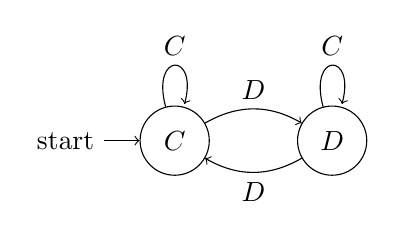
\begin{tikzpicture}[node distance=2cm]
  \node[state,initial] (s_0) {$C$};
  \node[state] (s_1) [right of=s_0] {$D$};

  \path[->] (s_0) edge [loop above] node {$C$} ();
  \path[->] (s_0) edge [bend left] node [above] {$D$} (s_1);
  \path[->] (s_1) edge [loop above] node {$C$} ();
  \path[->] (s_1) edge [bend left] node [below] {$D$} (s_0);
\end{tikzpicture}
  \centering
  \caption{Pavlov.}
\end{figure}

\begin{figure}
  \label{tftfigure}
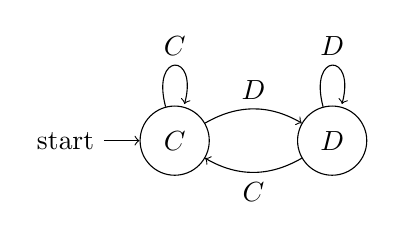
\begin{tikzpicture}[node distance=2cm]
  \node[state,initial] (s_0) {$C$};
  \node[state] (s_1) [right of=s_0] {$D$};

  \path[->] (s_0) edge [loop above] node {$C$} ();
  \path[->] (s_0) edge [bend left] node [above] {$D$} (s_1);
  \path[->] (s_1) edge [loop above] node {$D$} ();
  \path[->] (s_1) edge [bend left] node [below] {$C$} (s_0);
\end{tikzpicture}
  \centering
  \caption{Tit for tat.}
\end{figure}
  % \begin{tikzpicture}[scale=0.8, show background rectangle]
  %   \draw (0,0) -- (2,1);
  %   \draw (1,1) circle (3);
  %   \path[draw] (0,0) -- (1,1) -- (2,0);
  % \end{tikzpicture}


\begin{remark}
  Tit-for-tat, displayed in \cref{tftfigure}, is not evolutionarily stable. It has the stationary distribution $(\frac{1}{4},\frac{1}{4},\frac{1}{4},\frac{1}{4})$ in its own Markov chain, which has a payoff that is significantly smaller than $R$. This should be intuitive: if tit-for-tat makes one mistake, it goes into a defection cycle that it doesn't break out of until it makes a second mistake.

\end{remark}


\section{Proofs}

\subsection{Helpful Lemmas}

\begin{lemma}
  \label{limitvexists}
  The limit \begin{equation*}
    \lim_{p \to 0} v_{s_1}(s_2)
  \end{equation*}
  exists, for any strategies $s_1$ and $s_2$.
\end{lemma}
\begin{proof}
  Note that $v_{s_1}(s_2)$ is a weighted average of the rewards $R, T, S$ and $P$. Therefore, $S \leq v_{s_1}(s_2) \leq T$. \todo{eughhhh fix this somehow}
\end{proof}

\begin{lemma}
  \label{neverbetterthanr}
  For any strategy $s$,
  \begin{equation*}
    v_{s}(s) \leq R
  \end{equation*}
\end{lemma}
\begin{proof}
  For notational simplicity, we will let $s_1$ and $s_2$ be two copies of strategy $s$. Then, $v_{s}(s) = v_{s_1}(s_2) = v_{s_2}(s_1)$. By definition, we have
  \begin{equation*}
    v_{s_1}(s_2) = \sum \pi_{c_1,c_2} \cdot r(c_1,c_2)
  \end{equation*}
  and
  \begin{equation*}
    v_{s_2}(s_1) = \sum \pi_{c_2,c_1} \cdot r(c_2,c_1).
  \end{equation*}
  Note that $\pi_{c_1,c_2}$ and $\pi_{c_2,c_1}$ refer to the same state, so we thus have \begin{equation*}
    v_{s_1}(s_2) + v_{s_2}(s_1) = \sum \pi_{c_1,c_2} \cdot (r(c_1,c_2) + r(c_2,c_1))
  \end{equation*}
  which implies that \begin{equation*}
    v_s(s) = \sum \left( \pi_{c_1,c_2} \cdot \frac{r(c_1,c_2) + r(c_2,c_1)}{2} \right).
  \end{equation*}
  Now, note that $r(c_1,c_2) + r(c_2,c_1) \in \{R + R, S + T, T+S, P + P\}$. Since $P < R$ and $T + S < 2R$, we thus find that \begin{equation*}
    v_s(s) \leq \sum \pi_{c_1,c_2} \cdot R = R \sum \pi_{c_1,c_2} = R,
  \end{equation*}
  as desired.
\end{proof}

\subsection{Evolutionary Stability Implies Utilitarianism}

With these lemmas, we are now ready to prove our first theorem.

    \begin{proof}[Proof of \cref{evolutionarystable1}]
      Suppose that the strategy $s_1$ is such that it is \textit{not} true that \begin{equation*}
        \lim_{p \to 0 } v_{s_1}(s_1) = R
      \end{equation*}
      By \cref{limitvexists} and \cref{neverbetterthanr}, this assumption implies that the limit is strictly less than $R$. Define $\gamma = v_{s_1}(s_1)$. We thus know that \begin{equation*}
        \gamma < R.
      \end{equation*}
      
      We want to prove that $s_1$ is not evolutionarily stable. 
      
      To do that, we want to prove that for all $p_0, \epsilon_0 \in (0,1)$, there exists $p < p_0$ and $\epsilon < \epsilon_0$, such that $s_1$ is $\epsilon$-invadable. We choose $\epsilon = \epsilon_0 / 2$, and present a strategy $s_2$ that can invade $s_1$ for sufficiently small $p$.

      We create the strategy $s_2$ as follows. First, copy the entire $s_1$ machine into $s_2$. Suppose that the state corresponding to the start state of $s_1$ is $c$, and that the output at $c$ is $\alpha$, and that the state $s$ goes to upon perceiving the opponent move $\alpha$ is $c' = T(c, \alpha)$. Now, create two new states: $c_0$ and $c_1$. Define the transitions as \begin{align*}
        T(c_0, \alpha) &= c'\\
        T(c_0, \bar{\alpha}) &= c_1 \\
        T(c_1, \cdot) &= c_1
      \end{align*}
      and the outputs as \begin{align*}
        G(c_0) &= \lnot G(c_2)\\
        G(c_1) &= C.
      \end{align*}
      Let the start state of $s_2$ be $c_0$. 

      \begin{figure}
        \centering
        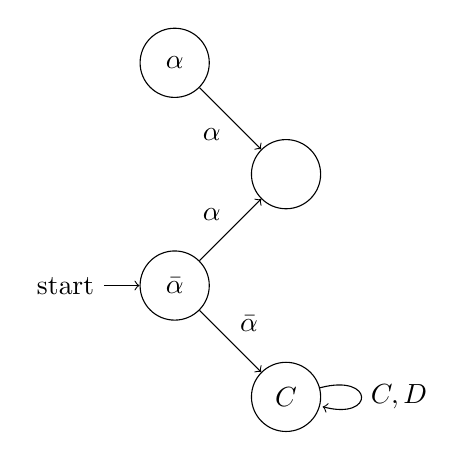
\begin{tikzpicture}[node distance=2cm]
          \node[state, initial] (c_0) {$\bar{\alpha}$};
          \node[state] (c_1) [below right of=c_0] {$C$};
          \node[state] (c_prime) [above right of=c_0] {};
          \node[state] (c) [above left of=c_prime] {$\alpha$};

          \path[->] (c_0) edge node [above right] {$\bar{\alpha}$} (c_1);
          \path[->] (c_1) edge [loop right] node [right] {$C,D$} ();
          \path[->] (c_0) edge node [above left] {$\alpha$} (c_prime);
          \path[->] (c) edge node [below left] {$\alpha$} (c_prime);
        \end{tikzpicture}
        \caption{Constructon of invasion strategy, used in the proof of \cref{evolutionarystable1}}
        \label{invasionstrategy}
      \end{figure}


      \begin{claim}
        \label{claimpayoffs}
        Given the above construction of $s_2$, the following inequalities hold:
      \begin{align*}
        v_{s_1}(s_1) &\leq (1-p)^2 \gamma + 2(1-p)p R + p^2  R \\ 
        v_{s_1}(s_2) &\leq (1-p) \gamma + p T \\
        v_{s_2}(s_1) &\geq (1 - p) \gamma  + p S \\
        v_{s_2}(s_2) &\geq (1-p)^{2} R + 2 (1-p) p (\tfrac{S + T}{2}) + p^2 \gamma .
      \end{align*}
      \end{claim}

      Before proving this claim, we will use it to finish our proof of \cref{evolutionarystable1}.

      Now, we simply compute $F(s_2) - F(s_1)$, which we want to show is greater than 0.
      \begin{align*}
        F(s_2) - F(s_1) &= \\
        &= (1 - \epsilon) \cdot v_{s_2}(s_1) + \epsilon \cdot v_{s_2}(s_2) - (1 - \epsilon) \cdot v_{s_1}(s_1) - \epsilon \cdot v_{s_1}(s_2) \\
        &= (1 - \epsilon) (\gamma + p(\ldots)) + \epsilon (R + p(\ldots)) - (1-\epsilon) (\gamma + p(\ldots)) - \epsilon (\gamma + p(\ldots)) \\
        &= \epsilon (R - \gamma) + p(\ldots)
      \end{align*}

      We know that $R - \gamma > 0$ by our initial assumption. Clearly, since $(\ldots)$ is some polynomial in $p$, given an $\epsilon$ we can find a sufficiently small $p$ such that the full expression is positive. This proves that $s_2$ can invade $s_1$, and thus, that $s_1$ is not $\epsilon$-invadable for this value of $p$. In conclusion, then $s_1$ is not evolutionarily stable, which concludes the proof of \cref{evolutionarystable1}.

    \end{proof}

    \begin{proof}[Proof of \cref{claimpayoffs}]
      We can prove this using either of the two definitions.
    \end{proof}

    \subsection{Evolutionarily Stable Strategies Exist}

    Unfortunately, we have no proof of \cref{pavlovtheorem}.

    We note that the $2R > T + P$ condition is necessary. Otherwise, the AllD strategy would be able to invade Pavlov. We see this by noting that $\lim_{p \to 0} v_{s_2}(s_1) = T + P$ if $s_2$ is AllD and $s_1$ is Pavlov, and that AllD is better against itself than Pavlov is against it.



    \section{Discussion of Model}



    \subsection{Other Potential Models}

    Right now we have only modeled noise in perception. One could think of another possible kind of noise: a ``failure of the mind,'' which perhaps could be modeled instead by a probability $p$ of being transported to any random state, instead. This would create ergodicity which is nice.

    \section{Appendix: Time average distributions}

    We might have periodicity, but for our purposes, we might as well extend the definition and look at periodic distributions as stationary too. The following two lemmas help with that.

    \begin{lemma}
      Given a starting distribution $v$ and a Markov matrix $M$, for every $\epsilon > 0$, there will exist a $k$ such that $|vP^{nk} - vP^{mk}| < \epsilon$ for all $n$ and $m$ $> 0$.
    \end{lemma}

    This proves that a Markov chain will always reach a periodic state.

    \begin{lemma}
      Suppose distributions form a chain $p_1 \to p_2 \to \cdots \to p_n \to p_1$. Then $\pi = \frac{p_1 + \ldots p_n}{n}$ is stationary.
    \end{lemma}

    This proves that we're able to talk about stationary distributions even when they don't really actually exist.


    \section{Appendix: Probablistic Automata}

    In this paper, we have considered strategies that make a deterministic move based on what they perceive. One could also imagine strategies that attaches a certain probability distribution to a perceived input, and chooses their next action based on that. In this appendix we show that these can be reduced to the deterministic ones, and thus that all results for the deterministic ones also hold for the probabilistic ones.

    Proof idea: we can use cycles in the Markov chain with n total outputs, x of which are to state 1, to model getting to state 1 with probability x / n. this assumes that the outputs are of low enough probability, which can be achieved by chaining together lots of (1-p) transitions, which go to 0.

    the hard part of this is showing that modifying the finite automaton like this won't hurt us. in fact, it would certainly not hurt us if not every state had to give an output. but that doesn't work for our model i think. so there are certainly things to think about here.

\end{document}